% Sparsification block — defense slides.
% Build:
%   - online: upload to overleaf.com, compile with XeLaTeX (UTF-8 + Cyrillic)
%   - local:  xelatex presentation.tex   (twice, for cross-refs)
% Required: ./slides/*.png in the same dir as this .tex (already in repo).

\documentclass[aspectratio=169,11pt]{beamer}

\usepackage{fontspec}
\usepackage{polyglossia}
\setmainlanguage{russian}
\setotherlanguage{english}
\setmainfont{Helvetica}
\setsansfont{Helvetica}
\setmonofont{Menlo}
\newfontfamily\russianfont{Helvetica}
\newfontfamily\russianfontsf{Helvetica}
\newfontfamily\russianfonttt{Menlo}

\usepackage{graphicx}
\usepackage{booktabs}
\usepackage{array}
\usepackage{xcolor}

% Theme — Madrid is built-in everywhere; switch to metropolis if you have it.
\usetheme{Madrid}
\usecolortheme{seahorse}

\definecolor{accent}{RGB}{52, 152, 219}
\definecolor{good}{RGB}{39, 174, 96}
\definecolor{bad}{RGB}{192, 57, 43}

\setbeamertemplate{navigation symbols}{}
\setbeamertemplate{caption}[numbered]
\setbeamercolor{title}{bg=accent, fg=white}
\setbeamercolor{frametitle}{bg=accent, fg=white}

\title[Спарсификация UNet]{Спарсификация UNet}
\subtitle{magnitude / 2:4 / structured + fine-tune}
\author{Курилов Олег}
\institute{Эффективные модели ML и архитектуры нейросетей}
\date{Апрель 2026}

\begin{document}

% ====================================================== Slide 1: Title
\begin{frame}
  \titlepage
\end{frame}

% ====================================================== Slide 2: Methods
\begin{frame}{Три метода и главные вопросы}
  \begin{columns}[T]
    \column{0.56\textwidth}
    \textbf{Что мерим}
    \vspace{0.3em}
    \begin{itemize}
      \item \textbf{Magnitude (L1)} --- занулить нижние $N\%$ весов по~$|w|$
      \item \textbf{2:4 semi-structured} --- 2~из~4 нулей вдоль input-channel
      \item \textbf{Structured channel} --- зануляем целые out-каналы
    \end{itemize}

    \column{0.44\textwidth}
    \textbf{На что смотрим}
    \vspace{0.3em}
    \begin{itemize}
      \item Качество --- Dice
      \item Скорость --- ms/img
      \item Память --- peak GB
      \item Восстановимо ли через fine-tune?
    \end{itemize}
  \end{columns}

  \vspace{1em}
  \begin{center}
    \footnotesize
    Бенчмарк: UNet 31\,M, Carvana val (400~images), A4000 16\,GB, fp16, bs=8.
  \end{center}
\end{frame}

% ====================================================== Slide 3: Quality envelope
\begin{frame}{Качество vs sparsity (без fine-tune)}
  \begin{center}
    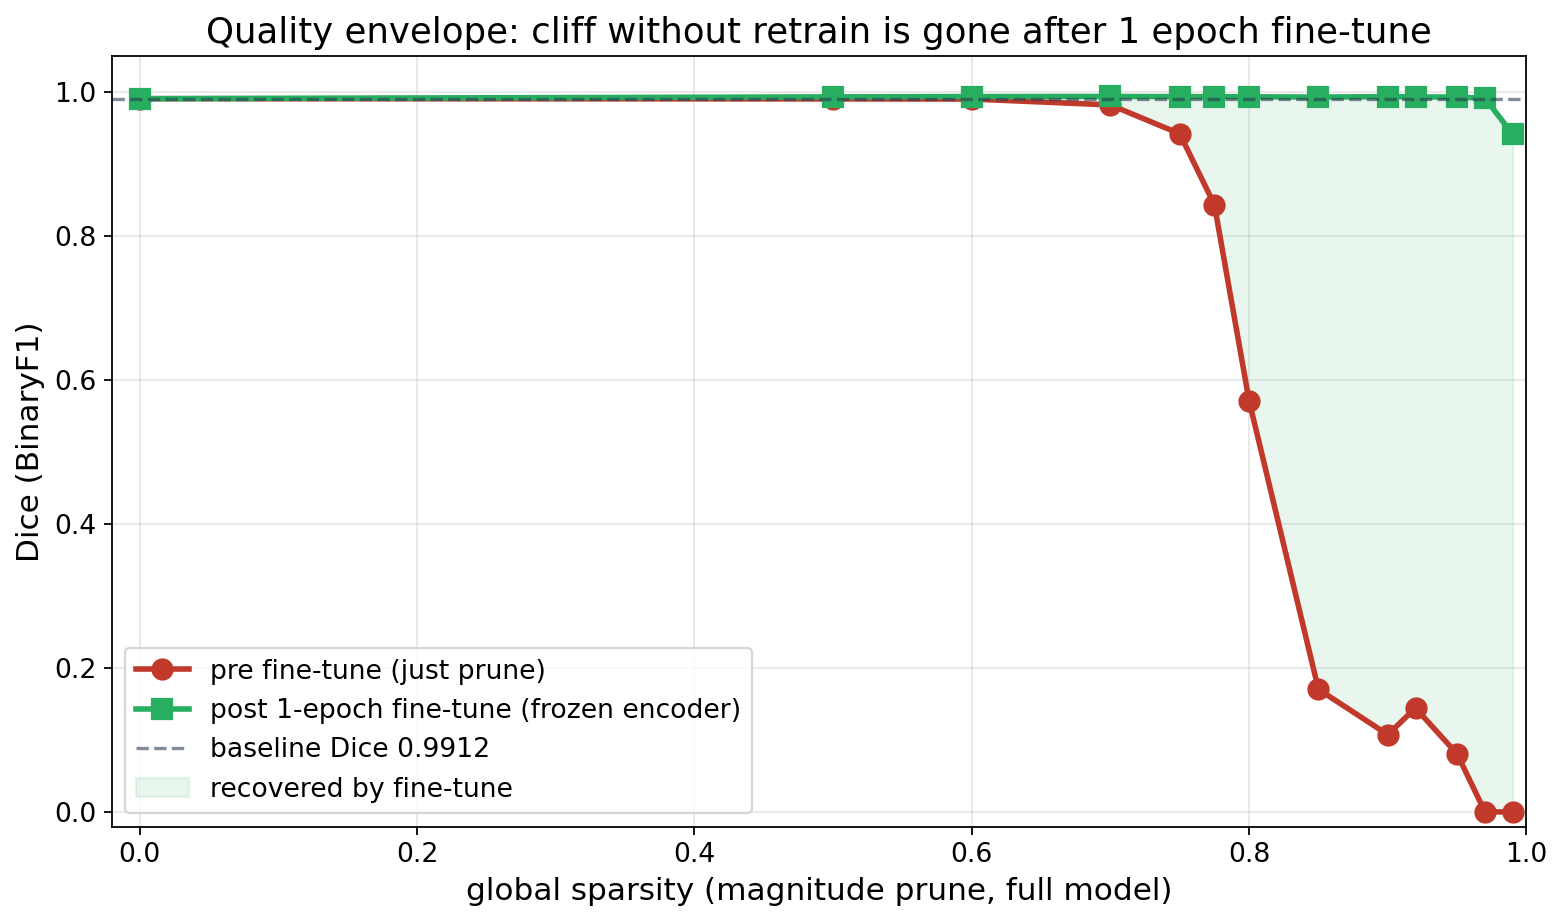
\includegraphics[width=0.78\linewidth]{slides/01_quality_envelope.png}
  \end{center}

  \textbf{\color{good} UNet выдерживает до 70\% magnitude sparsity почти бесплатно.}\\
  Cliff на 90\% --- без retrain модель ломается ($\textrm{Dice}=0.108$).
\end{frame}

% ====================================================== Slide 4: Fine-tune recovery
\begin{frame}{Fine-tune возвращает (и превышает) baseline}
  \begin{center}
    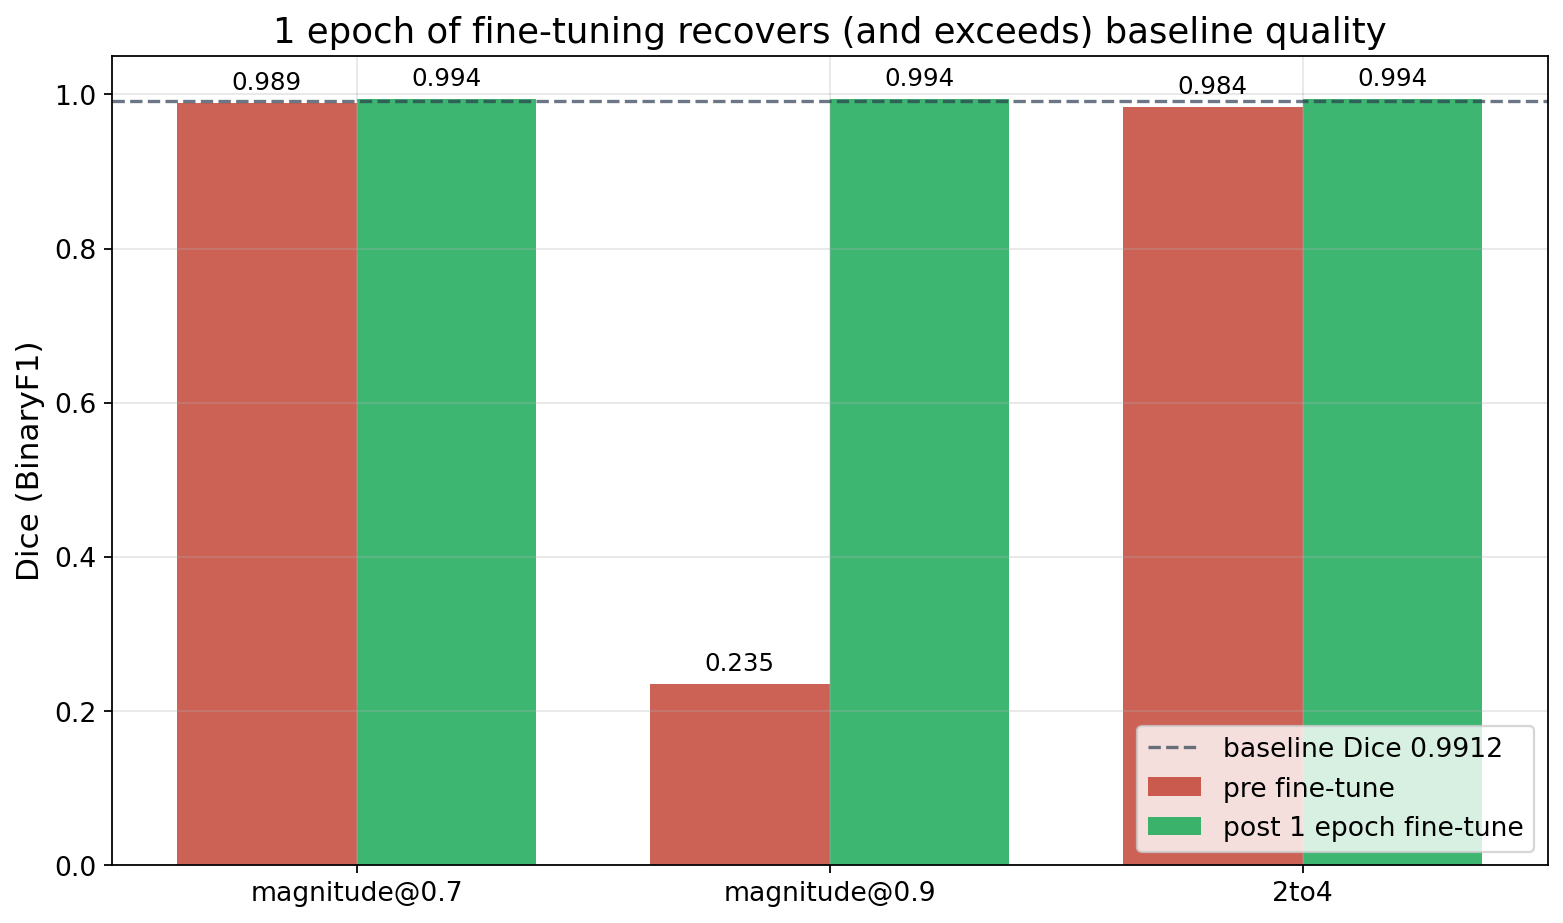
\includegraphics[width=0.82\linewidth]{slides/02_finetune_recovery.png}
  \end{center}

  \textbf{1~эпоха retrain (frozen encoder)} --- все три метода \textbf{выше} baseline 0.9912.\\
  Самый драматичный кейс: \texttt{magnitude@0.9} с {\color{bad}0.235} до {\color{good}0.994}.
\end{frame}

% ====================================================== Slide 5: Iterative + ASP combo
\begin{frame}{Iterative ladder и полный NVIDIA ASP combo}
  \begin{columns}[T]
    \column{0.5\textwidth}
    \begin{center}
      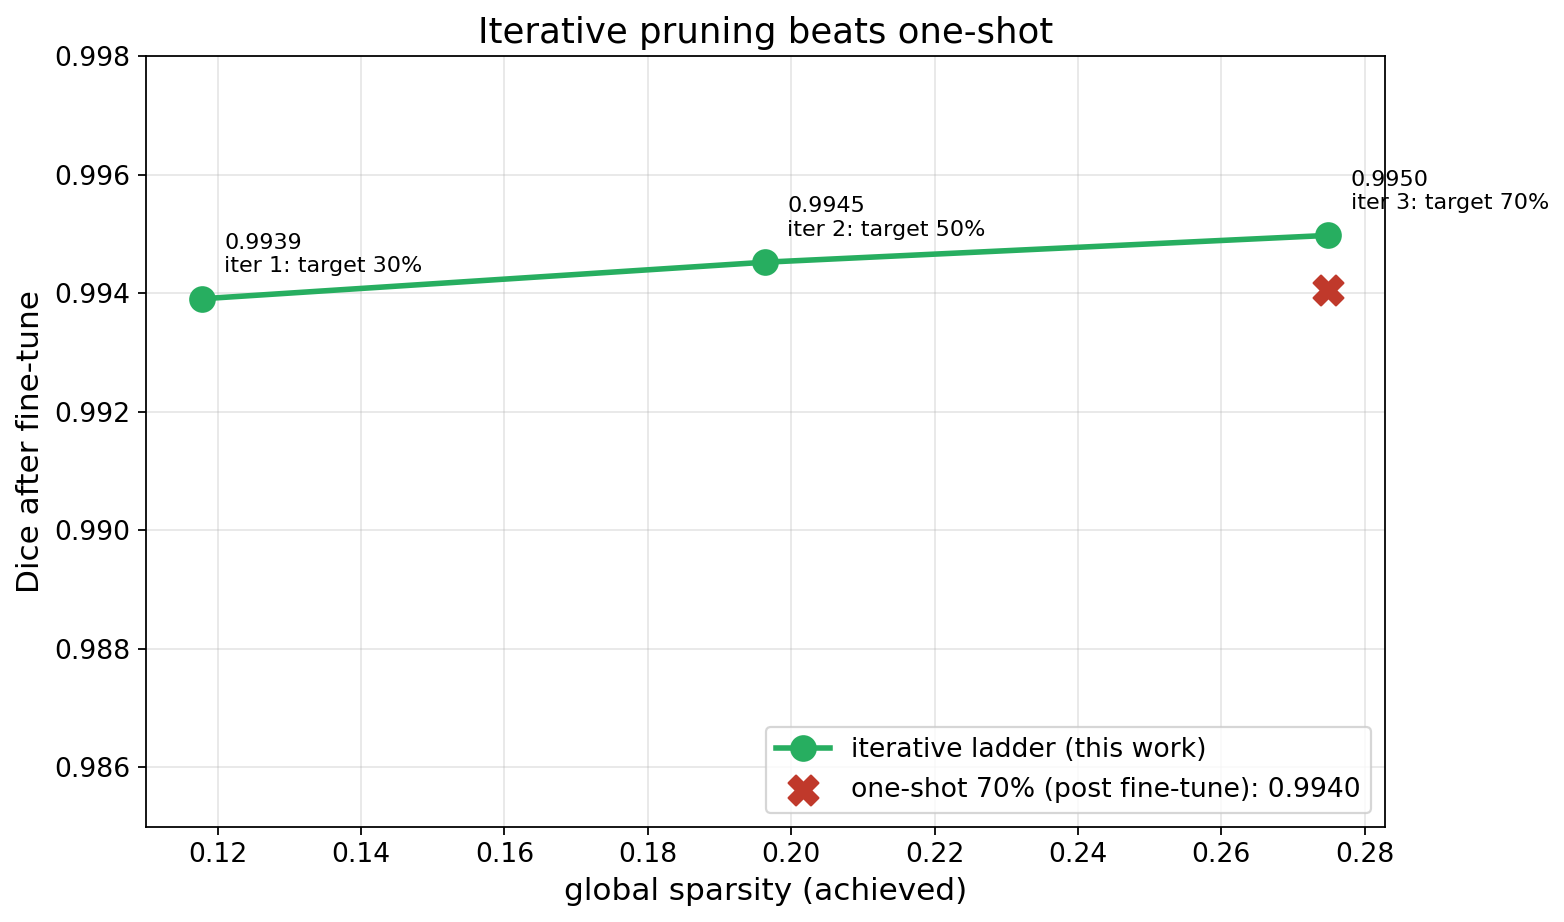
\includegraphics[width=\linewidth]{slides/03_iterative_vs_oneshot.png}
    \end{center}
    \footnotesize
    Gradual ladder $30\%\!\to\!50\%\!\to\!70\%$ даёт \textbf{Dice 0.9950}\\
    vs one-shot 0.9940 --- \textbf{+0.001}.

    \column{0.5\textwidth}
    \begin{center}
      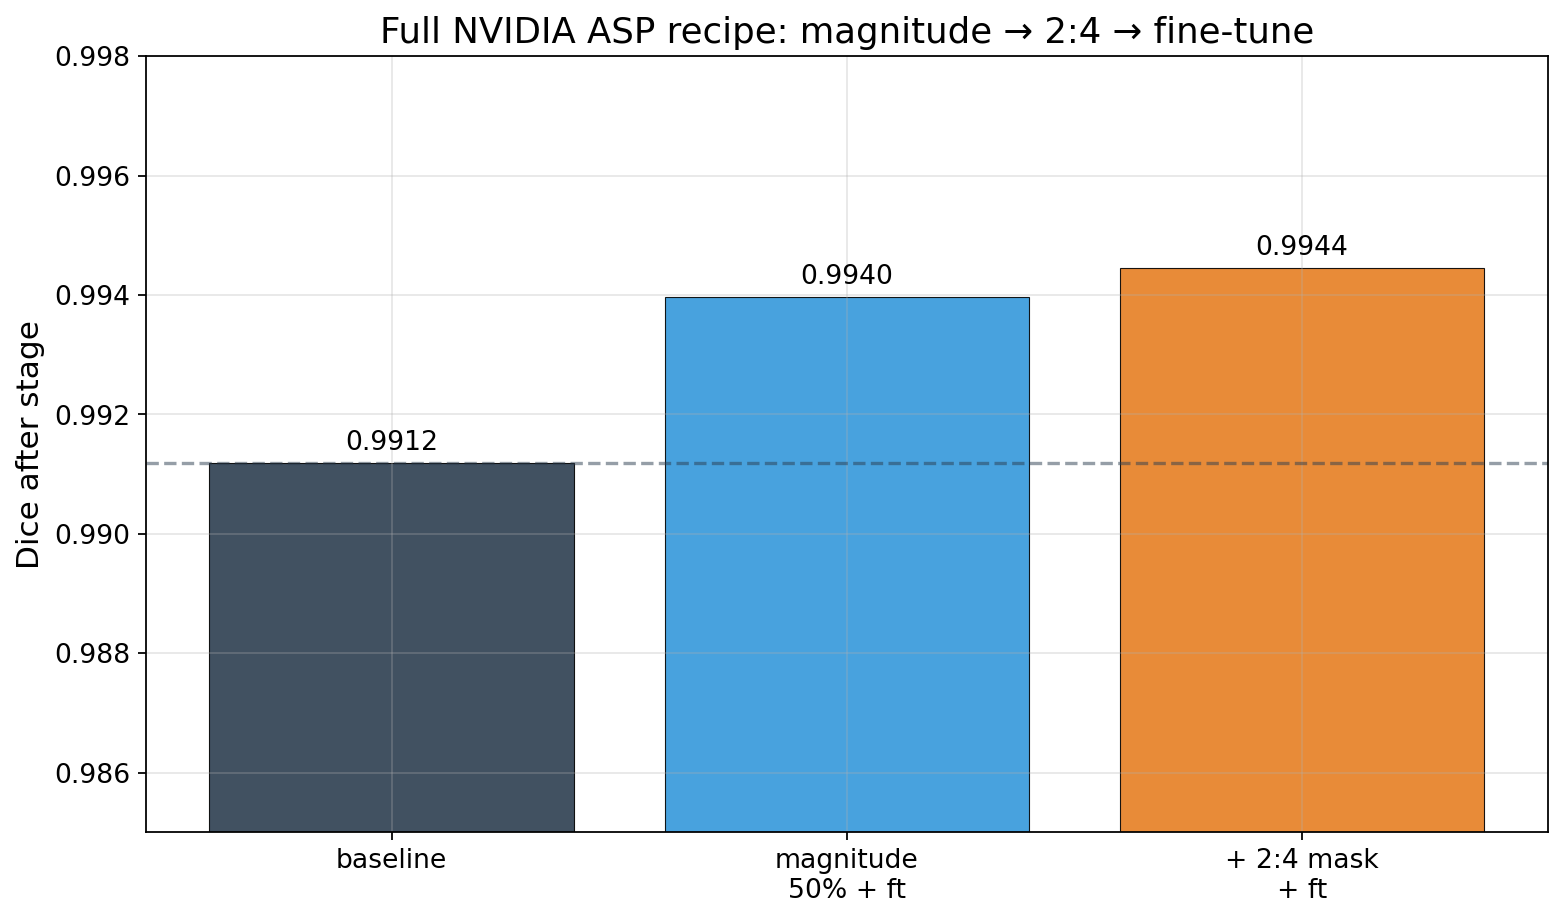
\includegraphics[width=\linewidth]{slides/04_asp_combo.png}
    \end{center}
    \footnotesize
    Полный ASP recipe: magnitude $\to$ 2:4 $\to$ fine-tune.\\
    Decoder Dice $0.9912 \to 0.9944$ при 24\% глобальной sparsity.
  \end{columns}
\end{frame}

% ====================================================== Slide 6: Profiler + cuSPARSELt
\begin{frame}{Реальный speedup: profiler и cuSPARSELt}
  \begin{columns}[T]
    \column{0.42\textwidth}
    \textbf{PyTorch Profiler} (4~активных батча):\\[0.4em]
    \begin{tabular}{lr}
      \toprule
      Конфиг & Self CUDA total\\
      \midrule
      baseline\_fp16  & 1.085\,s\\
      magnitude@0.5   & 1.078\,s\\
      2:4 (50\%)      & 1.076\,s\\
      \bottomrule
    \end{tabular}\\[0.5em]
    \footnotesize
    {\color{bad}\textbf{Разница $<1\%$}} --- 95\%~времени в \texttt{aten::conv2d}.
    Dense fp16 cudnn kernels не используют нули.

    \column{0.58\textwidth}
    \begin{center}
      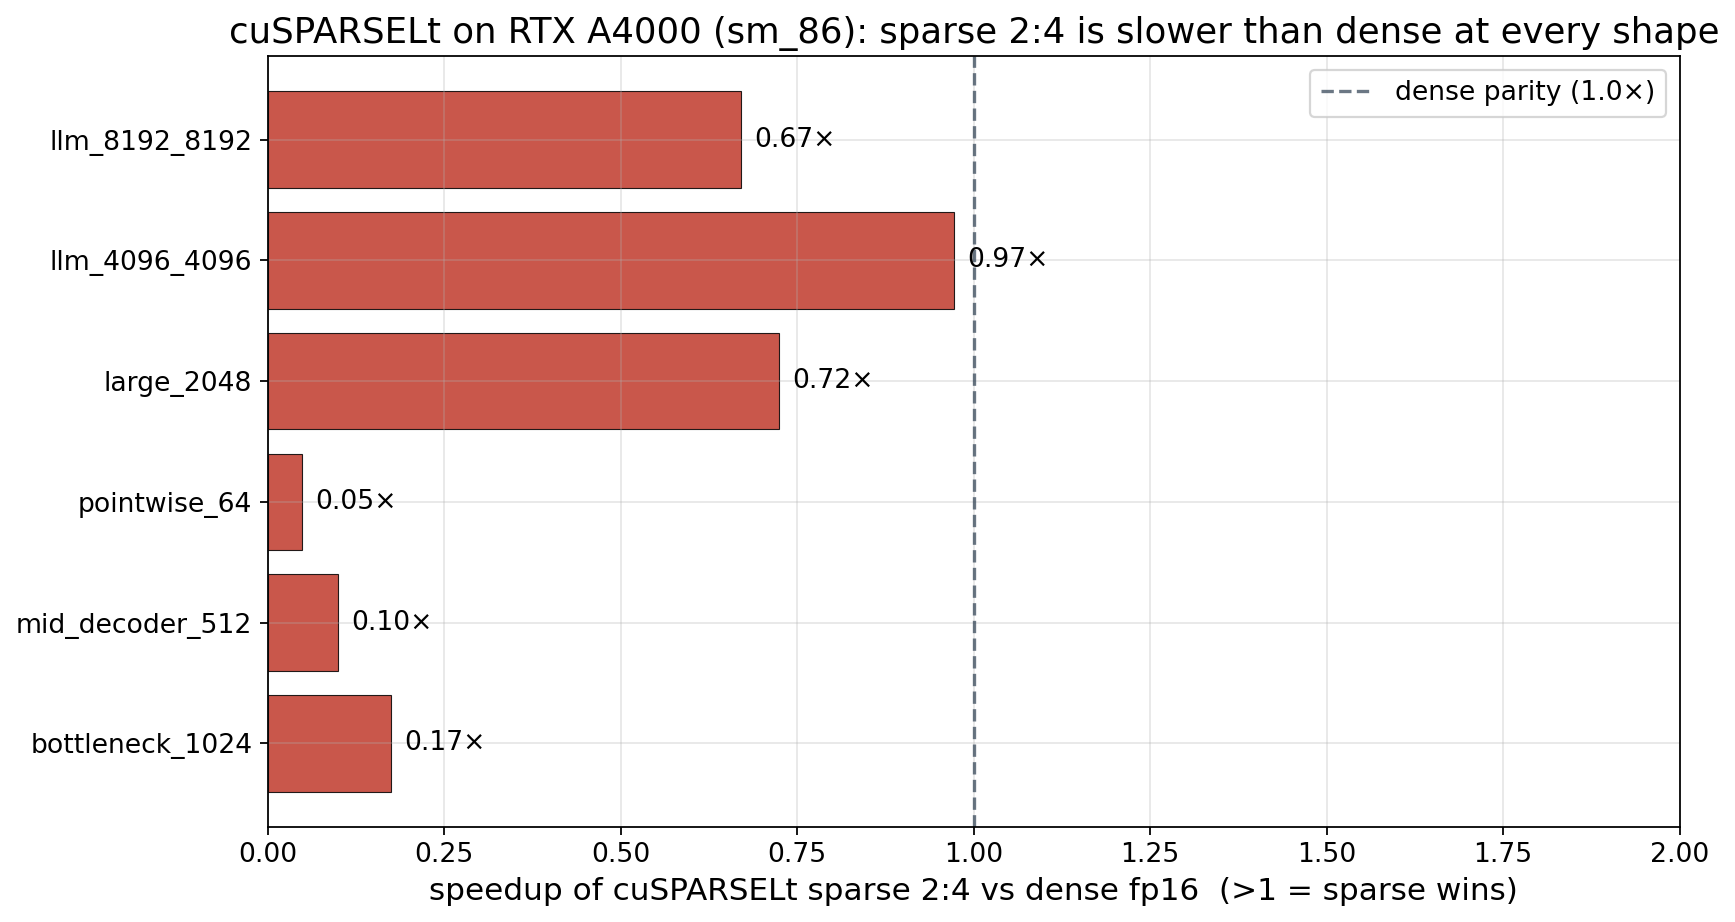
\includegraphics[width=\linewidth]{slides/05_cusparselt_speedup.png}
    \end{center}
    \footnotesize
    {\color{bad}\textbf{cuSPARSELt на A4000 не даёт speedup}} даже на LLM-shape.\\
    Hardware 2:4 path работает только на datacenter Ampere (sm\_80: A100).
  \end{columns}
\end{frame}

% ====================================================== Slide 7: Landscape + conclusions
\begin{frame}{Method landscape и выводы}
  \begin{columns}[T]
    \column{0.62\textwidth}
    \begin{center}
      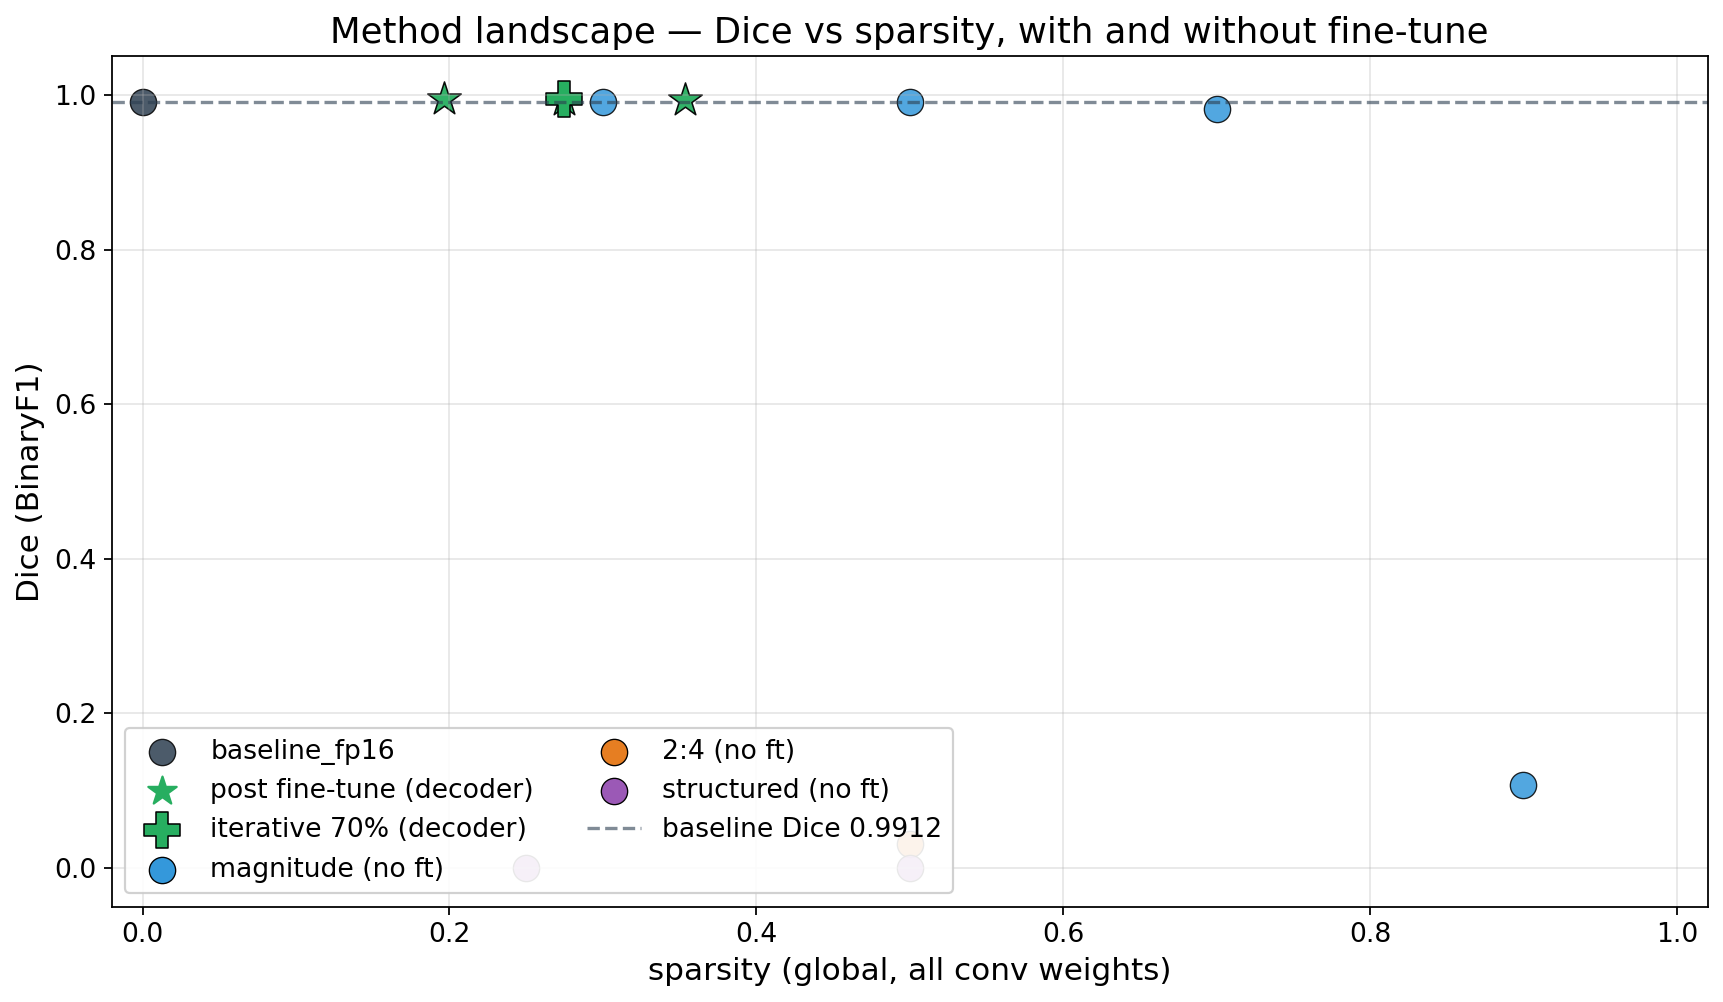
\includegraphics[width=\linewidth]{slides/06_method_landscape.png}
    \end{center}

    \column{0.38\textwidth}
    \footnotesize
    \textbf{Что узнали:}
    \begin{itemize}
      \item Качество --- 70\% magnitude бесплатно, через retrain --- выше baseline
      \item Скорость --- 0\% на dense kernels, отрицательная на cuSPARSELt
      \item Память --- идентична (zeros внутри tensor занимают то же место)
      \item Сэкономим только размер чекпоинта в sparse-формате
    \end{itemize}

    \vspace{0.5em}
    \textbf{Что дальше:}
    \begin{itemize}
      \item Physical channel removal (\texttt{torch\_pruning})
      \item Перенос на A100 $\to$ cuSPARSELt включится
      \item Combine с квантизацией --- ортогонально
    \end{itemize}
  \end{columns}
\end{frame}

% ====================================================== Backup
\begin{frame}{Спасибо. Артефакты}
  \footnotesize
  \begin{itemize}
    \item PR: \texttt{github.com/algorithm-pirogok/effml\_unet\_check/pull/1}
    \item Полный отчёт: \texttt{docs/sparsity.md} (200+ строк)
    \item 9 JSON: full benchmark, finetune, iterative, asp, cusparselt, memory, profile, smoke
    \item 6 фигур + 3 chrome traces (\texttt{ui.perfetto.dev})
  \end{itemize}

  \vspace{1em}
  \centering
  \textbf{Вопросы?}
\end{frame}

\end{document}
